%%%%%%%%%%%%%%%%%%%%%%%%%%%%%%%%%%%%%%%%%%%%%%%%%%
%
%  New template code for TAMU Theses and Dissertations starting Fall 2012.  
%  For more info about this template or the 
%  TAMU LaTeX User's Group, see http://www.howdy.me/.
%
%  Author: Wendy Lynn Turner 
%	 Version 1.0 
%  Last updated 8/5/2012
%
%%%%%%%%%%%%%%%%%%%%%%%%%%%%%%%%%%%%%%%%%%%%%%%%%%%
%%%%%%%%%%%%%%%%%%%%%%%%%%%%%%%%%%%%%%%%%%%%%%%%%%%%%%%%%%%%%%%%%%%%%%
%%                           SECTION IV
%%%%%%%%%%%%%%%%%%%%%%%%%%%%%%%%%%%%%%%%%%%%%%%%%%%%%%%%%%%%%%%%%%%%%


\chapter{\uppercase{Methodology}}



\section {The Problem}
Like any other program this bike sharing service also suffers few major problems. Bike rebalancing problem being the most important and significant of them all. This rebalancing problem occurs when a bike station is either full or empty and makes it difficult for users to rent or to park their rented bike. Thanks to the current prediction systems, it is possible to predict the usage of the bike share program and therefore allowing the users to have better experience of the bike share system. The objective is to make sure the users can walk to a bike docking station and find bikes to rent and also to discharge the rented bikes without having to wait for another user or going to another station to do that.

In order to find the problem and to set the goal of my thesis, first I did some statistical analysis on the bike share data and from those studies I saw that the distribution of the data is not balanced and same goes for gender distribution of the subscribers. Therefore, I tried to find a solution to overcome this two problem which is to forecast hourly rental bike demand for both men and women. I treated this problem as a regression forecasting with time series features and proposed Convolutional Neural Network (CNN) to do the forecasting which outperforms other traditional machine learning methods. I have used the data obtained from the City Bike system and weather data to forecast hourly rental demand of the Bike share system. 

\section{Datasets}

The goal of this thesis is to forecast bike demand using the users historical bike usage patterns along with the weather data and user's information in a time series arrangement. Therefore, this thesis attempts to answer the following questions : ``How many bikes are needed every hour?", ``Who are renting those bikes?", ``How weather is affecting the bike share usage?", ``Is it a holiday, weekend or normal weekday?". Therefore, datasets should contain three major information: 1) bike renting time and details, 2) users information, 3) weather data as well as 4) holiday/weekday-weekend information.

Collected dataset on the city bike share system contains details about the trip and the user who is renting it from January 2015 to July 2015. I have also collected weather datasets during that period and used January 2015 to June 2015 data sets to create the training set and the rest for testing set. 

Figure~\ref{datasets} shows the overview of the dataset preparation to build the forecasting model. Detailed information about the dataset extracting and processing will be discussed later in this chapter. 



\begin{figure}
\centering
\begin{adjustbox}{addcode={\begin{minipage}{\width}}
{\caption{Dataset Overview.}
\label{datasets}
\end{minipage}}}
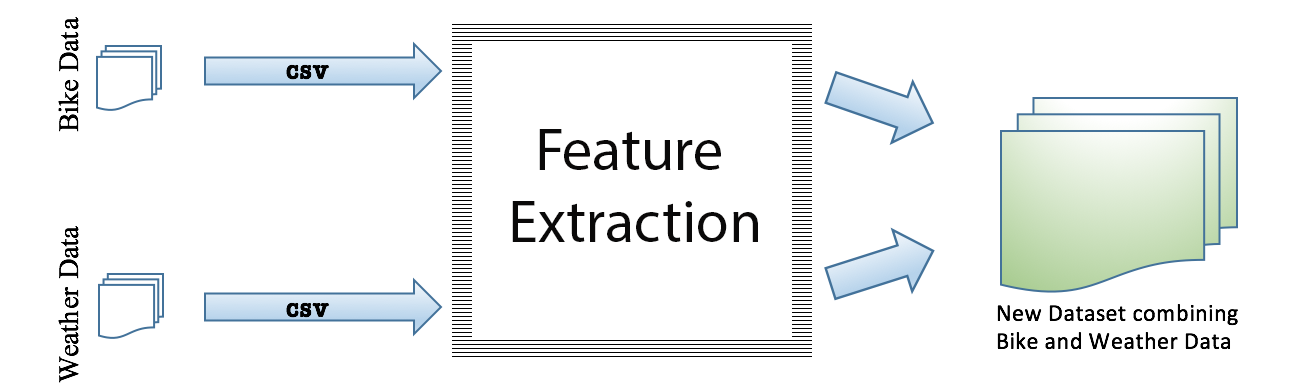
\includegraphics[scale=0.7]{figures/Dataset_overview.png}
\end{adjustbox}
\end{figure}


\subsection {New York City Bike Dataset}
\label{NYCdata}

The city bike system website provides historical datasets for all the researcher interested to carry out their research. This dataset is in CSV - comma separated values format. This dataset contains 6 key variables which are key to this thesis - `tripduration', `starttime', `stoptime', `usertype', `birthyear', `gender'.  This deals with the first two major topics which mentioned are above – 1) Bike renting time and details, 2) Users information. 

\begin{table}
\centering
\caption{Details of the Citi Bike Trip data }
\label{bikedata}
\vspace{1ex}
\begin{tabular}{||c||c |p{6.5cm} |c||}\hline
Field name & Type  &  Explanation & Information  \\\hline\hline
tripduration & Numeric & Duration of the ride in seconds & 1 \\\hline
starttime& Date& Start date and time of the trip  & 1 \\\hline
stoptime&Date &Stop date and time of the trip & 1 \\\hline
start station id&Numeric & Starting station id & 1 \\\hline
start station name& Character& Starting station name& 1 \\\hline
start station lattitude& Numeric& Starting station latitude& 1 \\\hline
start station longitude&Numeric &Starting station longitude & 1 \\\hline
end station id&Numeric &End station id & 1 \\\hline
end station name&Character &End station name & 1 \\\hline
end station lattitude&Numeric &End station latitude & 1 \\\hline
end station longitude&Numeric &End station longitude & 1 \\\hline
bikeid& Numeric& Bike identification& 1 \\\hline
usertype& Character& Type of user (Subscriber = Annual member, Customer = 24 hr/ 7 day pass) & 2 \\\hline
birthyear&Date &Users birth year & 2 \\\hline
gender& Numeric& Gender of the user (0=unknown, 1= male, 2= female)& 2\\\hline
\end{tabular}
\end{table}


The City Bike dataset has 3,379,904 entries of bike rental data and it all has the content showed in table~\ref{bikedata}.  Target bike rental dataset is then designed to get the time information, which is found by splitting the `starttime' into `hour', `month', `day'. Total number of rented bikes per hour can be then grouped in one field. Table~\ref{target_bikedata} shows the extracted details from those bike datasets which is then used for the experiment. 


\begin{table}[]
\centering
\caption{Target dataset of the Citi Bike trip data}
\label{target_bikedata}
\begin{tabular}{||l||l|l|l||}
\hline
Source                    & Name         & Type             & Information                            \\\hline\hline
\multirow{4}{*}{startime} & hourly count & numeric          & Total number of rented bike per hour   \\ \cline{2-4} 
                          & hour         & numeric          & Hour data                              \\ \cline{2-4} 
                          & day          & numeric          & Day                                    \\ \cline{2-4} 
                          & month        & numeric          & Month                                  \\ \hline
\multirow{2}{*}{usertype} & subscriber    & binary & Subscriber count                       \\ \cline{2-4} 
                          & customer     & binary & Customer count                       \\ \hline
birthyear                 & age          & numeric          & Age of the user                        \\ \hline
\multirow{3}{*}{gender}   & unknown      & binary & Unknown gender information of the user \\ \cline{2-4} 
                          & male         & binary & Male count                             \\ \cline{2-4} 
                          & female       & binary & Female count                           \\ \hline
\end{tabular}
\end{table}


\subsection {New York City Weather Dataset}
\label{NYCweatherdata}

For this thesis I have collected some historical New York City weather data from the NOAA (National centers for environmental information) website. From this dataset 8 key factors were chosen. These are – Date (Year, Month, Day), snow depth, snow fall, average wind speed, trip, precipitation. The target dataset from the weather data is shown in Table~\ref{target_weatherdata}.

\begin{table}[]
\centering
\caption{Target weather dataset}
\label{target_weatherdata}
\begin{tabular}{||c||l|l||}
\hline
Name               & \multicolumn{1}{c|}{Type} & \multicolumn{1}{c||}{Information}                         \\ \hline\hline
Year               & numeric                   & Year count                                               \\ \hline
Month              & numeric                   & Month count                                              \\ \hline
Day                & numeric                   & Day count                                                \\ \hline
Snow depth         & numeric                   & Snow depth level (in)                                    \\ \hline
Snow fall          & numeric                   & Snow fall rate (in)                                      \\ \hline
Average wind speed & numeric                   & Wind speed (mi)                                          \\ \hline
Temperature       & numeric                   & Temperature (F)                                          \\ \hline
Precipitation      & numeric                   & Rain, snow, sleet, or hail that falls to the ground (in) \\ \hline
\end{tabular}
\end{table}



\subsection {New York City Holiday Dataset}
\label{NYCholidaydata}


I have also collected dataset of the holiday during the period of Jan'2015 to July'2015 shown in figure~\ref{Holiday} and used it to build the training set of my model. There were 8 national holidays during the time period of the datasets related to this experiment of the year 2015 in USA. With this holiday weekend and weekday binary values will also be included in order to create the target dataset which is shown in 
Table~\ref{target_holidaydata}.  


\begin{figure}
\centering
\begin{adjustbox}{addcode={\begin{minipage}{\width}}
{\caption{Holiday list of NYC in 2015 (Jan-July) ~\cite{holidaysinnewyork}}
\label{Holiday}
\end{minipage}}}
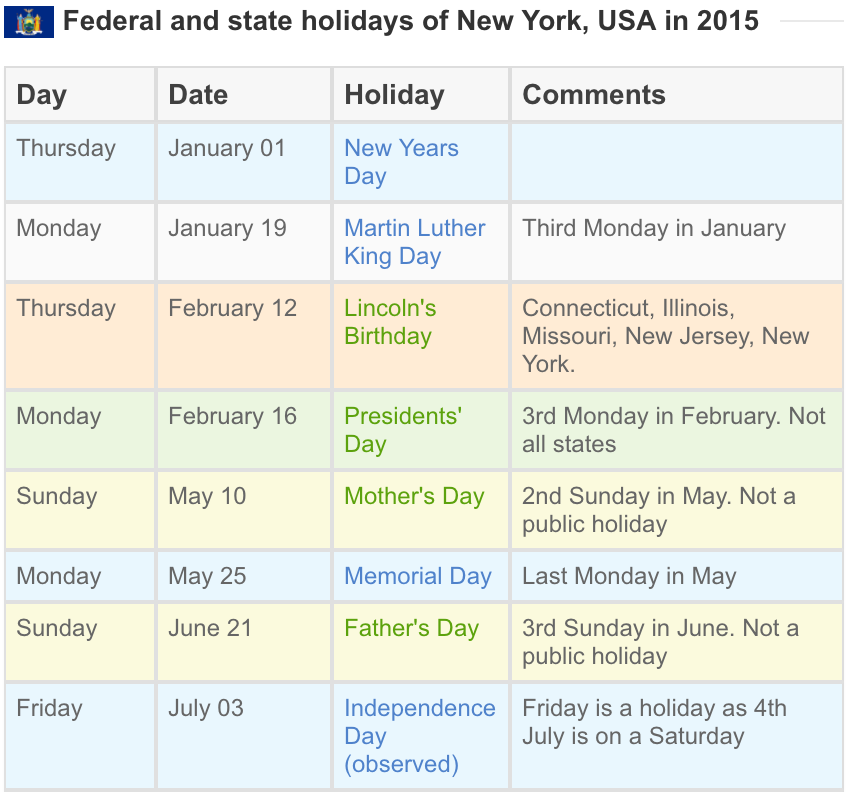
\includegraphics[scale=0.7]{figures/Holiday_nyc.png}
\end{adjustbox}
\end{figure}


\begin{table}[]
\centering
\caption{Target Holiday dataset}
\label{target_holidaydata}
\begin{tabular}{||c||l|l||}
\hline
Name                  & \multicolumn{1}{c|}{Type} & \multicolumn{1}{c||}{Information}           \\ \hline \hline
Holiday               & binary                    & Holiday binary value                       \\ \hline
Weekday               & binary                    & Weekday binary value                       \\ \hline
Weekend (not holiday) & binary                    & Weekend which are not holiday binary value \\ \hline
\end{tabular}
\end{table}



\section {Statistical Analysis}
\label{statistics}

In order to find the problem and to set the goal of my thesis, first I did some statistical analysis on the bike share data and from those studies I saw that the distribution of the data is not balanced and same for the distribution of the gender of the subscribers. Therefore, I tried to find a solution to overcome this two problem which is to forecast hourly rental bike demand for both men and women. I treated this problem as a regression forecasting with time series features and proposed Convolutional Neural Network (CNN) to do the forecasting which outperforms other traditional machine learning methods. I have used the data obtained from the City Bike system and weather data to forecast hourly rental demand of the Bike share system.


Getting more insights and understanding of the data before applying any machine learning tools is very important when it comes to forecasting. First we saw that there are two types of users in those data - subscribers and customers. So, then I tried to plot the trend of the bike share rentals between them. 


\begin{figure}
\centering
\begin{adjustbox}{addcode={\begin{minipage}{\width}}
{\caption{Customer vs Subscribers rental trend }
\label{custVSsubs}
\end{minipage}}}
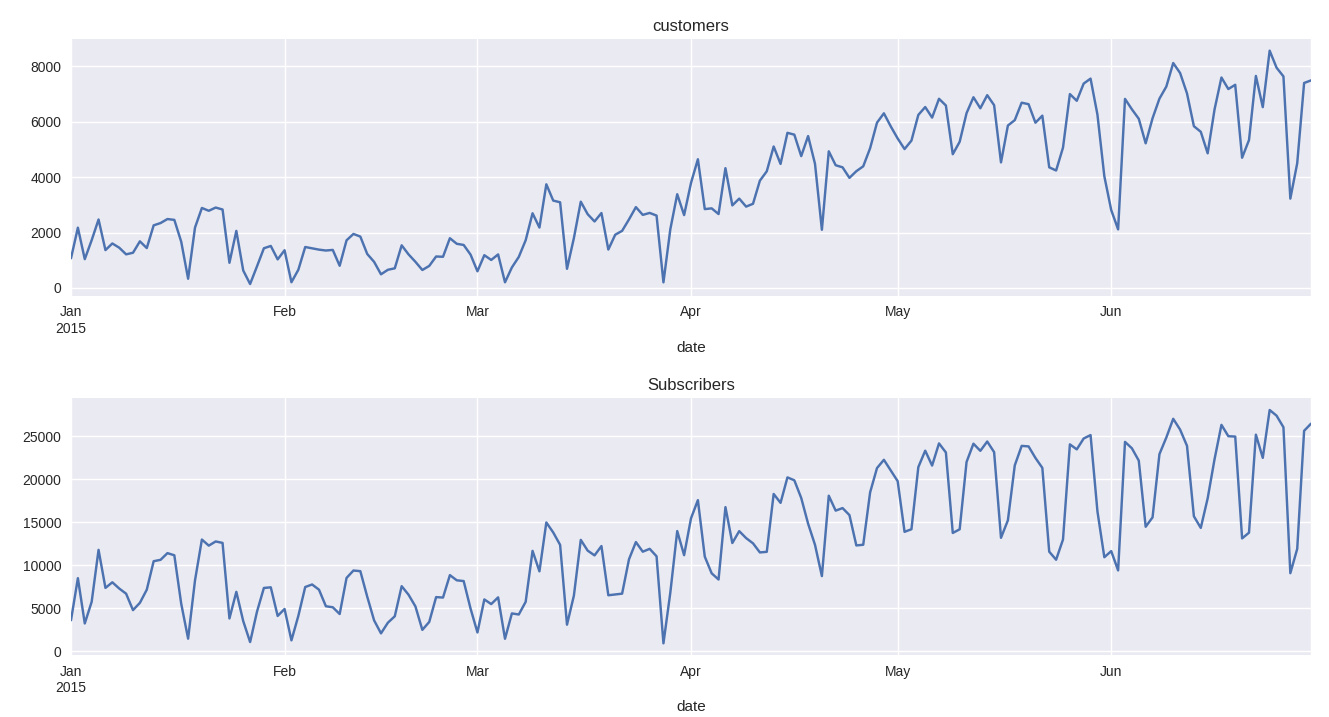
\includegraphics[ height=9cm, width=15cm]{figures/analysis/month.png}
\end{adjustbox}
\end{figure}

From this figure~\ref{custVSsubs} we can see that the customer count is almost less than $1/3$ in count and the distribution of the data is unbalanced which can be because of a lot factors like weekend, weekdays, good or bad weather, holiday etc. 


\subsection {Weekly Distribution}
\label{week}

To get more deep into this unbalanced distribution of the data, more deep analysis of the data is needed. Rather than getting the rental demand trend in monthly basis, weekly distribution is then applied. This time the weekly data is divided in gender basis, which is another important factor for this thesis. figure~\ref{maleVSfemale} shows the weekly average demand trend and from this figure we can see that rental demand significantly decreases when the weekend comes. This figure also shows a very valuable comparison between ``male" and ``female" rental demands. Females are $1/4$ less likely to rent a bike than males in New York City. There are also some unknown data which are the users who did not provide their gender details. The unknown data was really low during the weekdays but in the weekends the count rises high enough to even surpass female counts. Which also tells us that during weekends alot of people who are not subscribers, likes to roam around in the city using this bike sharing system. 

Doing daily analysis it was also found that the average number of bike rental demand per day for male is about $13$ thousands where for female it was $3,602$ and for unknown data it was around $2$ thousands. Another gender distribution is also shown in the figure~\ref{genderpie} where $69.3\%$ of rental data is provided by male and only $19.3\%$ of them are female, rest $11.4\%$ being the unknown categories. 
    


\begin{figure}
\centering
\begin{adjustbox}{addcode={\begin{minipage}{\width}}
{\caption{Male vs Female average rental demand per week}  
\label{maleVSfemale}
\end{minipage}}}
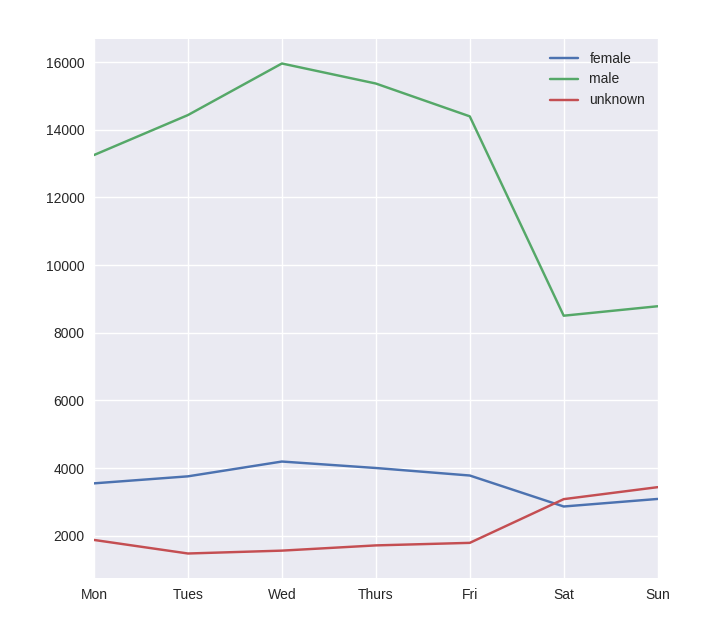
\includegraphics[scale=0.7]{figures/analysis/day.png}
\end{adjustbox}
\end{figure}



\begin{figure}
\centering
\begin{adjustbox}{addcode={\begin{minipage}{\width}}
{\caption{Gender distribution in rental demand of bikes}  
\label{genderpie}
\end{minipage}}}
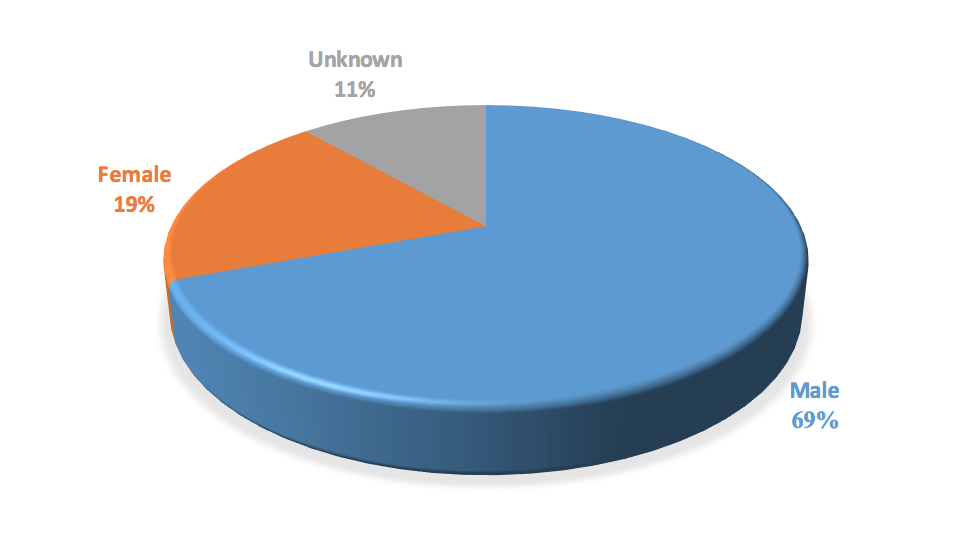
\includegraphics[scale=0.8]{figures/analysis/genderpie.png}
\end{adjustbox}
\end{figure}




\subsection {Trip Duration Frequency}
\label{trip}




A detailed analysis on the trip duration is also carried out in order to understand user behaviors behind renting bikes from this bike sharing system. There is also an extra charge after $30$ minutes of use of bike in one go for customers and after $45$ minutes for subscribers as shown in figure~\ref{duration} . So therefore, users are more likely to avoid this extra charge as one of the main reason behind using bike share system is to move around the city in an affordable way. But, from the data we observed an interesting tendency of the users. The maximum duration being $97744.35$ minutes which is either lost and then found or just an outlier in the data which we can neglect and minimum duration found is a minute. The mean duration is around $12.5$ minutes and most importantly more than $75\%$ is around $14$ minutes. So, from this we can realize that people mostly uses bike share program for short trips in the city.

\begin{figure}
\centering
\begin{adjustbox}{addcode={\begin{minipage}{\width}}
{\caption{Trip duration distribution between subscribers and customers} 
\label{duration}
\end{minipage}}}
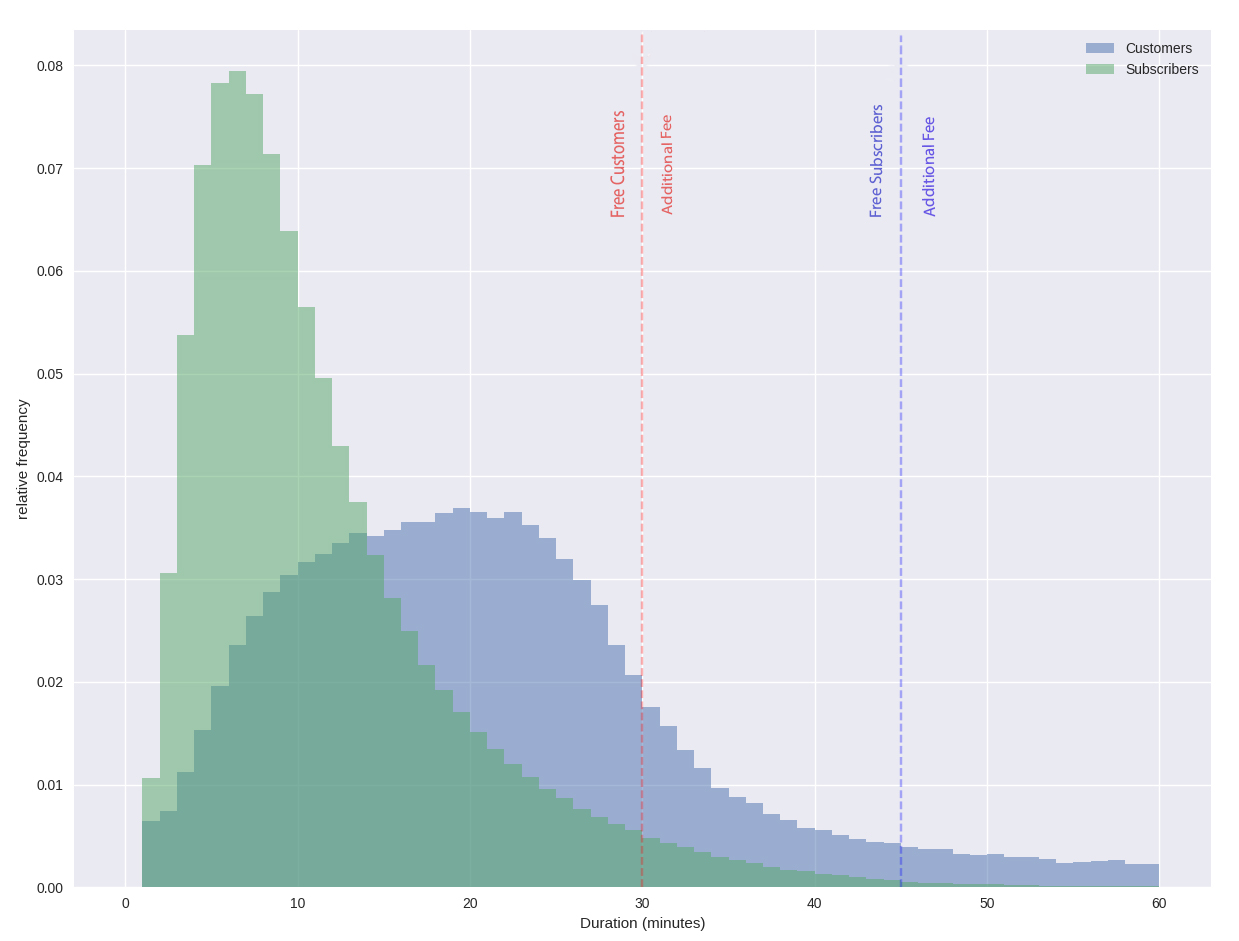
\includegraphics[width=1.0 \textwidth]{figures/analysis/duration.png}
\end{adjustbox}
\end{figure}

\subsection {Hourly Distribution}
\label{hourly}


Comparing the plots of the figure~\ref{hourly1} and figure~\ref{hourly2}, the shown graphs are based on the details about customers and subscribers and it shows that the pattern of the plot is noticeably different. ``Subscribers" who holds the annual pass for the bike share system displays `working' pattern. Which means the bike rental demand during the start and the end of the working hours are huge. Most people rents bike around 8:00 am and from 4:30 to 5:30 pm. ``Customers" who uses day or weekly passes shows random distribution of the data. It is also found that the maximum hourly demand of bikes in NYC in those time period is 3034 bikes and averages in about 540 bikes per hour, minimum being 1 bike.   

It is also found that the maximum age of a renter is a male being 77 years old and minimum is a female of 17 years old. The reason behind the minimum year is 17 is maybe because people under 17 do not hold credit cards. It is also very pleasing to see the mean values of age in general is 39 years. 



\begin{figure}
\centering
\begin{adjustbox}{addcode={\begin{minipage}{\width}}
{\caption{Hourly average rental demand in the City Bike trip data (Monday-Friday of Jan-June'2015)}  
\label{hourly1}
\end{minipage}}}
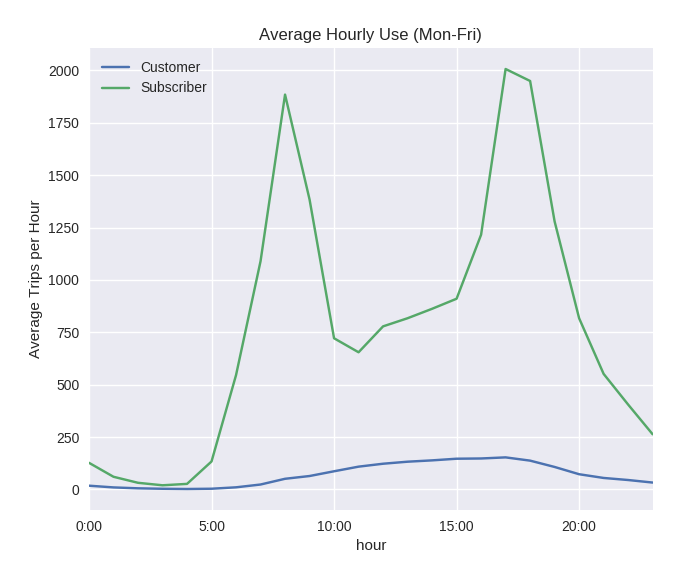
\includegraphics[scale=0.6]{figures/analysis/hourly1.png}
\end{adjustbox}
\end{figure}



\begin{figure}
\centering
\begin{adjustbox}{addcode={\begin{minipage}{\width}}
{\caption{Hourly average rental demand in the City Bike trip data (Saturday-Sunday of Jan-June'2015)}  
\label{hourly2}
\end{minipage}}}
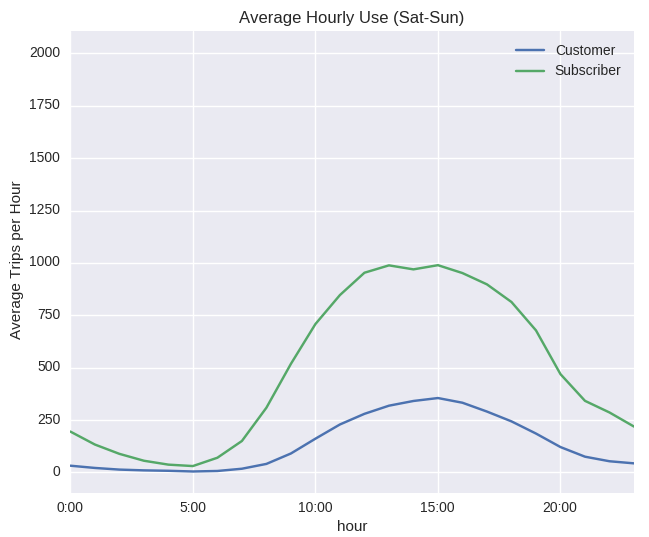
\includegraphics[scale=0.6]{figures/analysis/hourly2.png}
\end{adjustbox}
\end{figure}

After all this analysis of the data we can then conclude as the problem, where in these short bike trips between places it is very important to make sure users can rent and return a bike whenever they want. Therefore, the attempt of forecasting bike rental demand can play a vital role in order to predict the demand before it happens and thus rebalancing the whole system efficiently. Data also showed that customers normally uses bikes for short trips. So failing to deliver a rentable bike or a parking place in a desired station can cause the system to fail as a whole, as customers can sometimes just walk to the destination. Hence, it is very vital for a bike sharing program to make sure customers can get the best possible experience from it and stay subscribed. 


\section {Methodology}
\label{methodology}


Statistical results on the bike data prove that the distribution of the data is sometimes similar and therefore there is a big chance for researchers to find ways to improve the system. From the figure~\ref{maleVSfemale}, it shows the huge difference in rental demand count between male and female users in NYC. Therefore, there is big potential to increase the number of female users into this bike share system. In order to solve this matter, different bikes for different genders can be a very good option. By making the female bikes more appealing and colorful and also to design the bike to support female's body structure can provide better experiences for female users. 

This leads our main problem into two different problems. Forecasting and then providing enough bikes for both male and female users at any given hour. And the amount of female bikes needed can then also be determined from the rental demands of the female users. By doing this we can then forecast the adequate number of bikes needed also that every hour there will be enough bikes available for the users precisely.

\subsection{Convolutional Neural Network}
\label{CNNexpl}

Before discussing the problem and a way to solve it, it is necessary to understand how the Convolutional neural network works. As mentioned earlier in chapter 1 a CNN has three types of layers and the layer in use will decide the forward or back propagation is needed. A deep explanation of Forward and Back propagation of Convolutional layer and pooling layers are discussed below. 


\subsubsection{Forward Propagation}

Here it shows the computation of the layers in case of forward propagation :



\textbf {Convolutional Layers}:
To explain this section suppose we have $N \times N$ neuron layer trailed by the Convolutional layer. Then, the convolutional layer output $w$ will be $(N - m +1) \times (N - m + 1)$ if we use $m \times m$ filter. 

So, the pre-nonlinearity input to some unit $X_{ij}^{l}$  in the layer,  

$x_{ij}^{l}\sum_{a=0}^{m-1}\sum_{b=0}^{m-1}w_{ab}y_{(i+a)(j+b)}^{l-1}$ , this is done by summing up the weights by the filter sections from the earlier layer cells. After that the convolutional layer adds its non linearity – 
$y_{ij}^{l} = \sigma x_{ij}^{l}$.

\textbf {Max - Pooling Layers}: 
Max pooling layers basically takes some $k\times  k$ region and outputs the maximum single value for that region. For example, if they are getting input from a $N \times N$ layer then they will output a $ \frac{N}{k} \times \frac{N}{k}$ layer and using max function each $k \times  k$ block reduced to just a single value.

\subsubsection{Back Propagation}
The computation of the layers for back propagation :

\textbf {Convolutional Layers:}
Suppose the error function E and the error values at the convolutional layer is known. The error we know and the the calculation needed for the previous layer, with respect to each neuron output is the partial of E with respect to each neuron output$(\frac{\partial E}{\partial y_{ij}^l})$. By applying chain rule we can also compute the gradient. 

$\frac{\partial E}{\partial w_{ab}} = \sum_{i=0}^{N-m} \sum_{j=0}^{N-m} \frac{\partial E}{\partial x_{ij}^l} \frac{\partial x_{ij}^l}{\partial w_{ab}} = \sum_{i=0}^{N-m} \sum_{j=0}^{N-m} \frac{\partial E}{\partial x_{ij}^l} y_{(i+a)(j+b)}^{l-1}$. Here, we should add all $ x_{ij}^l $ where $ w_{ab}$ happens. We also need to calculate the deltas which the values of ${\frac{\partial E}{\partial x_{ij}^l}}$ by using chain rule again .

$\frac{\partial E}{\partial x_{ij}^l} = \frac{\partial E}{\partial y_{ij}^l} \frac{\partial y_{ij}^l}{\partial x_{ij}^l} =  \frac{\partial E}{\partial y_{ij}^l} \frac{\partial}{\partial x_{ij}^l} (\sigma (x_{ij}^l))= \frac{\partial E}{\partial y_{ij}^l}(\sigma{}' (x_{ij}^l))$. Therefore, deltas of the current layer can be very easily computed by using the derivative of the activation function $(\sigma{}' (x))$. Now the gradient can be computed with respect to the weights used by the convolutional layer. 

In addition, we need to propagate the errors back to its previous layer and by using chain rule once again we can compute that – 

$\frac{\partial E}{\partial y_{ij}^{l-1}} = \sum_{a=0}^{m-1} \sum_{b=0}^{m-1} \frac{\partial E}{\partial x_{(i-a)(j-b)}^l} \frac{\partial x_{(i-a)(j-b)}^l}{\partial y_{ij}^{l-1}} = \sum_{a=0}^{m-1} \sum_{b=0}^{m-1} \frac{\partial E}{\partial x_{(i-a)(j-b)}^l} w_{ab}$

From this we can see the convolution effect. The equation above is valid for points which are atleast $m$ away from the left and top edge. And to fix that we simply need to fix that with zeros and it will be simply a convolution using $w$ which is flipped by both the axes. 


\textbf {Max - Pooling Layers}:
The backpropagated error for the max pooling layer is sparse. As mentioned earlier pooling layer do not do any learning themselves. And in forward propagation blocks $k \times k$ is reduced to its single value. Then this value attains error calculated from back propagation from the previous layer. Therefore, the value just gets forwarded to the place where it came from.


\subsection{Problem Formulation}
\label{Problem}

In this section, previously introduced hourly bike rental demand forecasting will be studied more using the datasets and based on the analysis mentioned earlier. Hourly bike rental demand forecasting has a goal to predict the bike rental demands based on the historical rental demand and the proposed method is a regression problem with the time series features. 


Time series is an arrangement of measurements taken at controlled points in time (usually equally spaced manner). It was originally developed by applying statistical methods in the field of econometrics, which is then used in a variety of fields like physics, ecology and engineering. The main focus of the time series analysis is prediction by producing precise forecasting of forthcoming measurements from a given series. Forecasting using time series takes the form-

$Y= b_0 + b_1 X_1+b_2 X_2+...+b_n X_n$

where, $X_1,X_2,... ,X_n$ are the independent variables, $b_0$ is the intercept and $b_1,b_2,... ,b_n$ are the coefficients represents the contribution of $X_1,X_2,... ,X_n$ .

As we are treating our problem as a time series regression problem, so to do forecasting we need to use related historical rental demand data. For the target value Y which is the bike rental demand, we then have to design a model for $Y_t$ which is the value of rental demand Y at any given time t. Before building the model architecture we need to realize that this time series are related to its previous observations. Therefore, to build a model for $y_t$ we need to take all the previous values of $y_t,. . .,y_n$ as it has an effect on it. So our model should look like – 

$Y_t= df_{model} (Y_{t-1},Y_{t-2},...,Y_{t-n})$

Here, $df_{model}$ is the demand forecasting model which is dependent on the previous $Y_t$ values such as $Y_{t-1}$ means last hours rental demand, $Y_{t-2}$ means the rental demand of two hours ago from $t$ hour and so on. 

But this $df_{model}$  also depends on the other two datasets mentioned earlier, weather and holiday. So, after taking those in account we can rewrite our equation into something like this :

 
$Y_t= df_{model} (W_{t-1},W_{t-2},...,W_{t-n})$

Where, $W_{t-1}$ is the combination of all the features that came to consideration while forecasting bike rental demand $Y$ at time $t-1$, such as rental demand, weather, holiday. 

After selecting this features and modeling the problem, restructuring was done to treat this features as image pixel features. The reason is to treat this bike rental demand forecasting problem as an image evaluation problem figure~\ref{imagebike}.    


\begin{figure}
\centering
\begin{adjustbox}{addcode={\begin{minipage}{\width}}
{\caption{Comparing Image pixel with Bike rental demand sample } 
\label{imagebike}
\end{minipage}}}
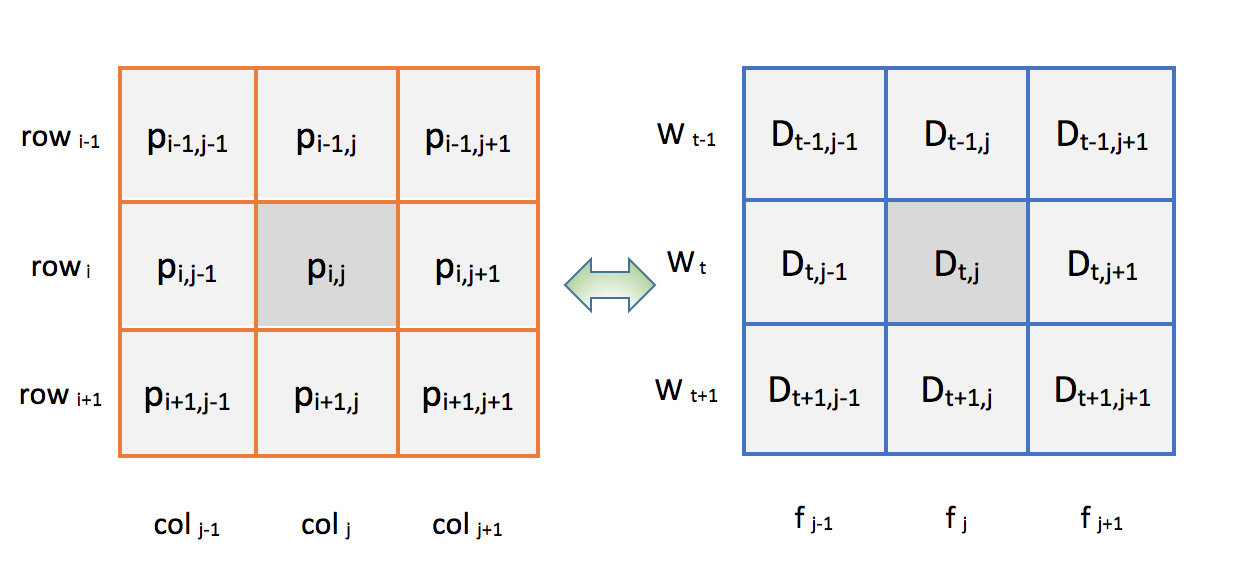
\includegraphics[scale=0.7]{figures/imagebike.png}
\end{adjustbox}
\end{figure}


In an image analysis problem, image samples contains many many pixels and these pixels are surrounded by a lot of pixels that has influence on the target pixel. For a $3\times3$ example as shown in the left sub figure of figure~\ref{imagebike} a target image pixel $p_{i,j}$ is bounded by the related pixels. In this sub figure the rows are mentioned as $i$ and columns as $j$. 

Likewise, for our model to forecast demand in a particular hour $D_{t,j}$ , which is surrounded by some historical hour values as shown in the combined hours field of Table~\ref{datacombo}. So, the demand $D_{t,j}$ is then relies on the combined related feature value $W_t$ (at time t) and $f_j$ is factor $j$. Proposed CNN model is then applied to this time series feature data by reflecting the relations with the image sample and thus dealing this bike rental demand forecasting as an image processing problem. 




\subsection{Model Structure}
\label{structure}

To build the forecasting model to estimate hourly rental bike demand a Convolutional Neural Network model is applied. The structure of a CNN based regression model is shown in figure~\ref{Framework}.


\begin{figure}
\centering
\begin{adjustbox}{addcode={\begin{minipage}{\width}}
{\caption{Structure of a CNN based regression model } 
\label{Framework}
\end{minipage}}}
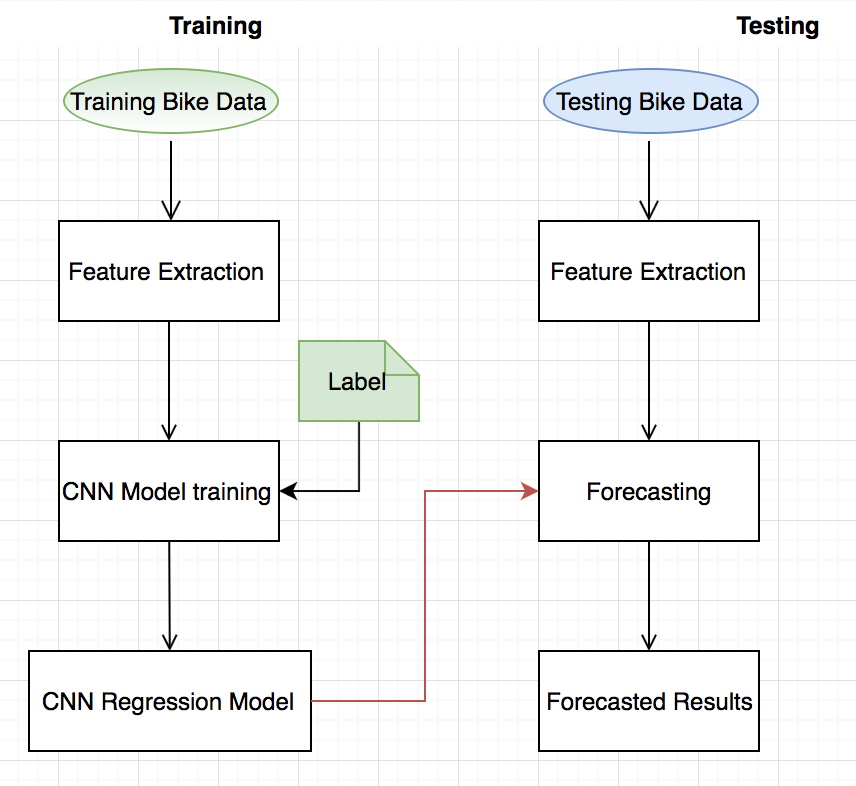
\includegraphics[scale=0.7]{figures/Framework.png}
\end{adjustbox}
\end{figure}


Like any other machine learning method there are two different fragment of it, one is training and the other is testing. For the training part, the datasets gets isolated by keeping the related fields which affects the bike rental demands as features through the feature extraction methods. Afterwards, multiple structures of CNN is analyzed in order to find the best structure of the model. Three different structures of CNN is applied with different convolutional layer count shown in figure~\ref{CNN1}, figure~\ref{CNN2} and figure~\ref{CNN3}. In the next section, this model is implemented on the testing set to forecast the hourly rental demand and then evaluated with four different evaluation matrices to calculate their effectiveness. 



\begin{figure}
\centering
\begin{adjustbox}{addcode={\begin{minipage}{\width}}
{\caption{5 Layer CNN } 
\label{CNN1}
\end{minipage}}}
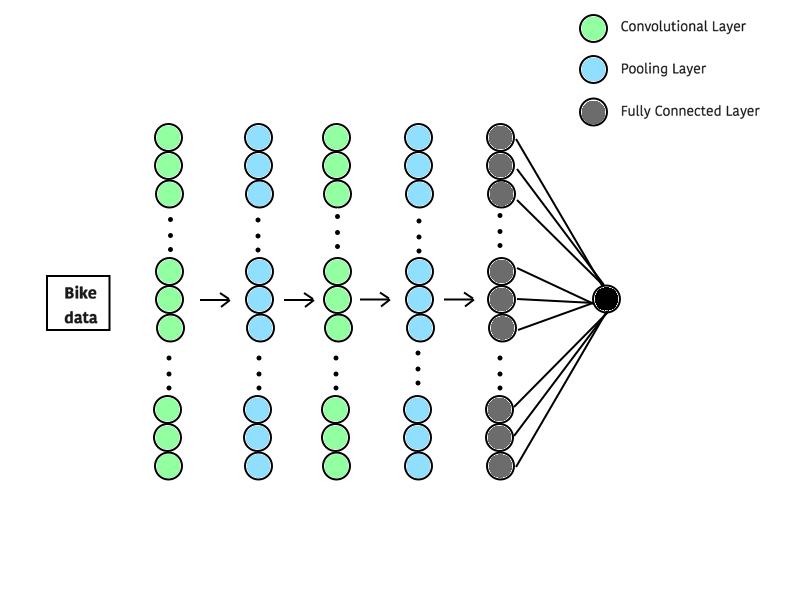
\includegraphics[scale=0.4]{figures/cnn5.png}
\end{adjustbox}
\end{figure}

\begin{figure}
\centering
\begin{adjustbox}{addcode={\begin{minipage}{\width}}
{\caption{6 Layer CNN } 
\label{CNN2}
\end{minipage}}}
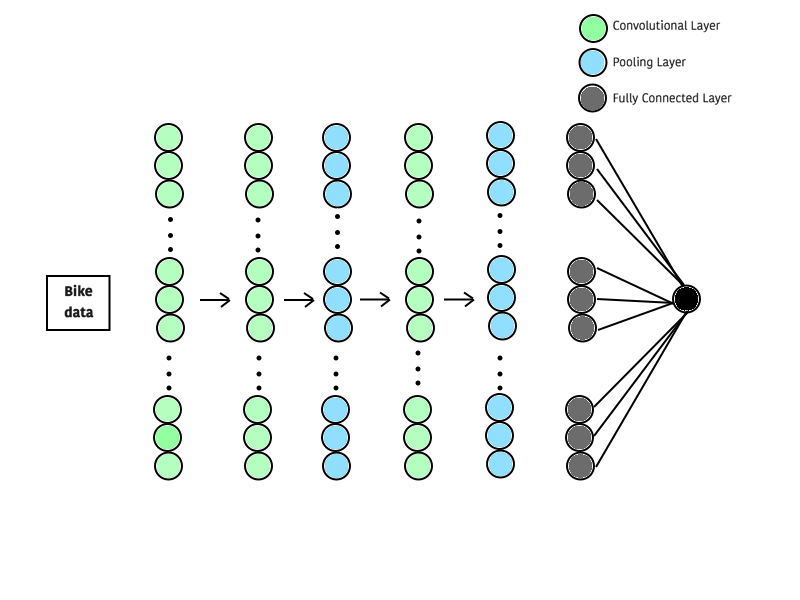
\includegraphics[scale=0.4]{figures/cnn6.png}
\end{adjustbox}
\end{figure}


\begin{figure}
\centering
\begin{adjustbox}{addcode={\begin{minipage}{\width}}
{\caption{7 Layer CNN } 
\label{CNN3}
\end{minipage}}}
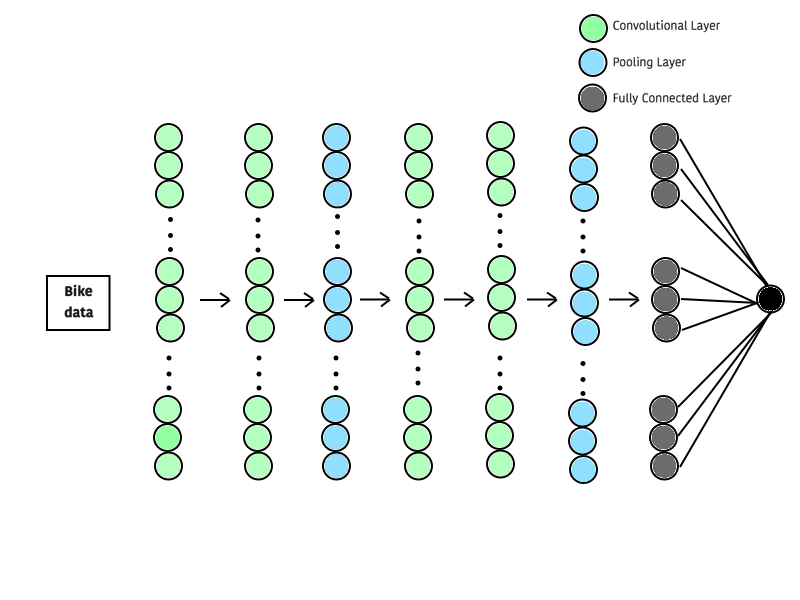
\includegraphics[scale=0.4]{figures/cnn7.png}
\end{adjustbox}
\end{figure}

In figure~\ref{CNN1} there are 5 layers in that CNN structure where, one convolutional layer is connected to one pooling layer which is then connected to another convolutional layer and then again to another pooling layer and finally to a fully connected layer. In figure~\ref{CNN2} there is one extra convolutional layer and in figure~\ref{CNN3} two extra convolutional layer from the 5 layer CNN and thus constructs 6 Layer CNN and 7 Layer CNN respectively. 














%

%%%%%%%%%%%
%
%As highlighted in the previous chapter, analogous to conditioning in probability, DST also has its conditional notions for evidence updating~\cite{CHRISMAN1995}. In this chapter, the basic conditional notions and their implications are presented providing insight into their behavior and the reason behind the choice of the particularly proposed conditional chosen in this thesis.
%
%
%
%
%The most acknowledged DST conditional notions are the DS conditionals~\cite{SHAFER} and FH conditionals~\cite{FaginH}. Although both methods are similar in some respects, FH conditionals possess more intuitive properties (as will be shown in subsequent sections) applicable for hard/soft fusion applications. 
%
%keywords= \lbrace {data handling;diseases;medical computing;regression analysis;social networking (online);Centers for Disease Control and Prevention;H1N1;ILI activity;Twitter data;autoregression models;flu trend prediction;influenza epidemics;influenza-like illness activity data;public health authorities;social network enabled flu trends framework;Correlation;Data models;Delay;Medical services;Predictive models;Real time systems;Twitter}, 
%doi={10.1109/INFCOMW.2011.5928903.
%
%Furthermore, although not expressly treated in this work, Wickramaratne et al. solved the converse problem determining the events which contributed to a particular conditional result. This is obtained by treating the converse CCT problem~\cite{Wickra4}. This is valuable in analyzing how sensitive the knowledge base is to incoming conditioning evidence.
%
%
%
%\section {Conditional Notion Characterization}
%
%An extensive review  was carried out by Kimala and Yamada on DST and the different conditional notions available in literature~\cite{Kimala2008}. However in any application (including soft/hard data fusion), one must consider the suitability of the conditional notion to be applied. 
%
%
%One driver behind our choice of appropriate DST conditional is the natural transition between the DST conditional and Bayesian conditional notions. This is vital because we expect our fusion strategy to be seamlessly integrated with the several approaches applied for dealing with hard data obtained from sensor networks as these methods are well grounded. However, there has been some works on finding the connection between Bayesian and DS theory~\cite{Pearl:1988}. We will now discuss two DST conditional notions arguably the most popular in literature.
%
%
%\subsection{DS or FH Conditionals?}
%The idea behind the DS conditionals is this: assuming we have access to a mass function $m(\textbf{.})$ and some new evidence signifying the occurrence of an event \textit{A}. Since we are confident this event has occurred, we can represent this event using the mass function with one focal element (\textit{A}), the DS conditional with respect to $A$ is given as $m(\extbf{.} \vert A) = (m \oplus m_{A})(\textbf{.})$, where $\oplus$ is the DCR. Technically, DS conditionals may be seen as an extension of Bayesian conditioning only when all focal elements are singletons, but not in general; a property possessed by most if not all other conditional notions. Furthermore, in applications where contradictory evidence are to be combined (as may be encountered in a battlefield scenario), the DCR will produce counterintuitive results. This is therefore a major drawback to the application of DS conditionals.
%
%A rigorous characterization of FH conditionals  has been carried out in which it they are shown to be a true generalization of the Bayesian conditionals~\cite{Fagin89uncertaintybelief, FaginH}. In the Bayesian context, a probability function  is bounded by its inner and outer measures~\cite{FaginH}. In the DS conditional context the probability function induced by inner and outer measures are the belief and plausibility functions respectively. The connection between both Bayesian and DS notions is immediately apparent; DS notions generalize Bayesian notion since inner and outer measures induced by probability functions `map' to DS theoretic belief and plausibility functions.  The fact that currently, no other conditional possesses this feature ~\cite{Fagin89uncertaintybelief} makes the FH our prime choice for the  hard/soft data fusion framework. In conclusion, the DS conditionals can also be constrained by certain paradoxes like \textit{the sure thing principle}, a constraint the FH conditions are able to circumvent~\cite{FaginH}.
%
%In light of the aforementioned reasons, in the following sections, discussions will be restricted to the FH conditionals and their characterizations only.
%
%\section{Characterizing the Conditional Core}
%
%Here we proceed to introduce the \textit{conditional core theorem} (CCT), which provides a theoretical framework with necessary conditions for an element to belong to the conditional core. 
%
%\subsection{Basics}
%
%%\theoremstyle{definition}
%\begin{definition}{(Inner and Outer Sets).}
%Given a BoE $\mathcal{E} \equiv \lbrace \Theta, \mathfrak{F}_{\Theta}, m_{\Theta(\textbf{.})} \rbrace$, and a conditioning event $A \subseteq \Theta$ satisfying $A \in \^{\mathfrak{F}}_\Theta$, the inner and outer sets are defined thus:
%\begin{eqnarray}
%in(A) &\equiv& \{B \subseteq A \vert B  \in  \mathfrak{F} \} \quad and \\
%out(A) &\equiv& \{B \subseteq A \vert B \cup C \in \mathfrak{F}, \quad \emptyset \neq B, \quad \emptyset \neq C \subseteq \overline A\}.
%\end{eqnarray}
%
%\end{definition}
%
%respectively. Also Also for indexes $\mathcal{I}$ and $\mathcal{J}$ spanning in$(A)$ and out$(A)$, we may define collections consisting or arbitrary unions of in(A) and out(A) as:
%\begin {eqnarray}
%IN(A) &=& {\{B \subseteq A \vert B = \bigcup_{\substack{
%   i \subseteq \mathcal{I} }} C_i, C_i \in in(A) \}\\
%OUT(A) &=& {\{B \subseteq A \vert B = \bigcup_{\substack{ j \subseteq \mathcal{J} }}, C_j, C_j \in out(A) \}
%\end{eqnarray}
%
%in$(A)$ connotes the set of focal elements contained in $A$, out$(A)$ contains the focal elements that intersect with but are not contained in $A$, IN$(A)$ and OUT$(A)$ contain arbitrary unions of elements of in$(A)$ and out$(A)$ respectively as shown in Figure ~\ref{inOutA}. $in(A)$, $out(A)$ and their union are significant factors contributing to our main result as shall be shown.
%
%\begin{figure}
%\centering
%\begin{adjustbox}{addcode={\begin{minipage}{\width}}
%{\caption{Pictorial representation of in(A) and out(A)~\cite{Wickra4}.}
%\label{inOutA}
%\end{minipage}}}
%\includegraphics[scale=0.8]{figures/inOutA.png}
%\end{adjustbox}
%\end{figure}
%
%
%%\theoremstyle{definition}
%\begin{definition}{(Straddled Mass).}
%Given a BoE $\mathcal{E} \equiv \lbrace \Theta, \mathfrak{F}_{\Theta}, m_{\Theta(\textbf{.})} \rbrace$, and two arbitrary subsets $A\subseteq \Theta$ and $B \subseteq \Theta$, the term:
%\begin{eqnarray}
%$\mathcal{S} (A;B)$  &= \displaystyle \sum_{\substack{\emptyset \neq X \subseteq A; 
%\emptyset \neq Y \subseteq B}}
%{m_{\Theta}(X \cup Y),
%\end{eqnarray}is the ``straddle'' mass, and is the cumulative mass of propositions straddling $A$ and $B$. 
%\end{definition}
%
%\begin{definition}{(Conditional Belief).}
%The conditional belief of any arbitrary proposition/hypothesis $B \subseteq \Theta$ is given by:
%\begin{eqnarray}
%Bl_{\Theta}(B \vert A) = \frac{Bl_{\Theta}(A \cap B)}{Pl_{\Theta}(A) - \mathcal{S}(\overline{A}; A \cap B)}
%\end{eqnarray}
%
%\end{definition}
%$A$ denotes the conditioning event satisfying $A \in \^{\mathfrak{F}}_{\Theta}$. The proof of this can be inferred from the relationship $Pl_{\Theta}(A) - \mathcal{S}(\overline{A}; A \cap B) = Bl_{\Theta}(A \cap B) + Pl_{\Theta}(A \cap \overline{B})$.
%
%
%\subsection{Conditional Core Theorem (CCT)}
%Having introduced the basics, we now introduce the theorem which specifies the constraints necessary to ascertain whether an element belongs to the conditional core:
%
%\begin{theorem}[Conditional Core Theorem]
%\label{CCT}
%For an arbitrary BoE $\mathcal{E}_{\Theta} = \lbrace \Theta, \mathfrak{F}_{\Theta}, m_{\Theta}(\textbf{.}) \rbrace$, the conditional mass function $m_\Theta(\textbf{.} \vert A)$  must satisfy the following constraints:
%\begin{eqnarray}
%m_{\Theta}(B \vert A) > 0 \leftrightarrow B \in in(A) \quad \textit{or} \\\nonumber
%B \in in(A) \cup OUT(A);
%\end{eqnarray}
%
%where $A$ defines our conditioning event satisfying $A \in \^{\mathfrak{F}}_{\Theta}$.
%\end{Theorem}
%
%This formulation is intuitive because it breaks down the FH notion and   provides insight into the generation of conditional focal elements, and also contains the tools needed to understand how the structure of the core affects the conditional core. The proof of the CCT is however not at all trivial and is hence not included in this thesis. The reader is referred to~\cite{Wickra3} where a through proof is detailed.
%
%Here, a short application example is employed to further expatiate on the CCT. Considering a variation of the illustration in~\cite{Wickra4}, we assume a situation assessment problem where objects that cross the perimeter of a military facility are to be identified. The objects of interest include:
%
%\begin{center}
%
%F \equiv Fighter; M\equiv Bomber;   T \equiv Tank;   S \equiv Soldier;   O \equiv Other
%\end{center}
%
%Furthermore, each class (with exception of $O$) can be subdivided as either $F \equiv Friendly$ or $E \equiv Enemy$ resulting in the following $FOD$
%
%\begin{center}
%$\Theta = \{F_E, F_F, M_E, M_F, T_E, T_F, S_E, S_F, O\}$
%\end{center}
%
%where for instance, $F_e \equiv \textit{enemy fighter jet}, M_f \equiv \textit{friendly bomber} \dots $
%
%BoE  = $\mathcal{E} = \{\Theta, \mathfrak{F} ,m\}$ is the available evidence, where:
%
%\begin{center}
%$\mathfrak{F} = \{M_E, M_F, S_F, (F_E, S_E), (M_E, T_E, O), \Theta \};$
%
%$m(B) = \{0.1, 0.1, 0.1, 0.2, 0.2, 0.3\}.$
%\end{center}
%
%Hence, the core of our BoE on ground, $\mathfrak{F}$, consist singleton propositions like $M_f$ signifying \textit{friendly bomber} and some composite statements like $\lbrace F_e, S_e \rbrace$ signifying \textbf{either}  \textit{enemy fighter jet} \textbf{or} \textit{enemy soldier}.
%
%\begin{table}
%\caption{Table showing conditional elements with non-zero mass. The conditional masses are generated via computation of the mass function given the conditioning event $A=\lbrace F_E , F_F , M_E , M_F , O\rbrace$}.
%\label{example}
%\centering
%\begin{tabular}{||c|c ||c |c||}\hline
%$B$ & $m(B\vert A)$  &  $B & $m(B\vert A)$  \\\hline\hline
%$M_E $&1/9 &$ (M_F, F_E)$& 2/63$ \\
%$M_F$ &1/9 & $(M_E,O)$ & 2/63 \\
%$(M,O)$ &2/63&  $(F_E,M,O)$ & 8/315$\\
%$(M_E,F_E)$ &  2/63 & $(M_E,F_E,O)$& 8/315 \\
% $A $ & 3/5 & &\\\hline
%\end{tabular}
%\end{table}
%
%Assuming we need to update the BoE to reflect incoming intelligence  of $(A = F,M,O)$ supporting  aerial intruder/objects. First we derive:
%$$ in(A) = \lbrace M_E, M_F \rbrace $$
%$$ out(A) = \lbrace F_E. (M_E,O), (F,M,O) \rbrace $$
%$$ IN(A) = \lbrace M_E, M_F, M \rbrace $$
%$$ OUT(A) = \lbrace F_E, (M_E, O), (F_E, M_E,O), (F,M,O) \rbrace $$
%
%Furthermore
%$$ \mathcal{B} = \lbrace (F_E,M_E), (F_E, M_F), (M_E, O), (F_E, M_E, O), (M, O), (F_E, M, O), A \rbrace $$ represents the set of propositions that can be found in $X \cup Y$ where $X \in in(A), Y \in OUT(A)$. Therefore based on the CCT, the concatenation of $\mathcal{B}$ and $in(A)$ constitutes the conditional focal elements, $\mathfrak{F}_{\vert A}$ (i.e. $\lbrace X \subseteq \Theta  \vert X \in in(A)$ or $X \in \mathcal{B} \rbrace $. Table ~\ref{example} shows the computed conditional masses using the CCT. From the above example, some inferences can be made:
%
%\begin{enumerate}
%\item When the evidence on ground $(B)$ is conditioned with $A = (F,M,O)$; hypotheses in favor of only aerial objects stay in the conditional core (e.g. $M_E$), whereas hypothesis supporting non-aerial objects  (e.g. $S_F$) are 'marginalized' out of the conditional core.
%
%\item Regarding the generated conditional focal set:
%	\begin{enumerate}
%	\item The propositions $\{F_E, S_E\}$ and $\{F_E, M_F\}$ receive the unconditioned mass of proposition $\{F_E, S_E\}$
%	\item The reason why generated the mass of $\{F_E, S_E\}$ does not move into just $F_E$ is because our unconditioned core $			\mathfrak{F}$ does not contain any singleton propositions favoring $F_E$, the same can be said for $\{F_E, M_E, O\}$. However 		propositions $F_E$ and $\{M_E, O\}$ do transition into $\{M_E, F_E, O\}$
%	\end{enumerate}
%\end{enumerate}
%
%The intuitiveness of the CCT is immediately apparent, as it shows the  logical coherence behind the allocation of conditional masses. Suppose the conditioning event was more precise (e.g. $A = \lbrace F,M_E, O\rbrace$), we would obtain the following:
%
%$$ in(A) = \lbrace M_E \rbrace $$
%$$ out(A) = \lbrace F_E. (M_E,O), (F,M_E,O) \rbrace $$
%$$ IN(A) = \lbrace M_E \rbrace $$
%$$ OUT(A) = \lbrace F_E, (M_E, O), (F_E, M_E,O), (F,M_E,O) \rbrace $$
%$$ \mathcal{B} = \lbrace (F_E,M_E),  (M_E, O), (F_E, M_E, O), (F, M_E, O) \rbrace $$
%$$\mathfrak{F}_{\vert A} = \lbrace M_E, (F_E,M_E),  (M_E, O), (F_E, M_E, O), (F, M_E, O) \rbrace $$
%
%
%Table~\ref{exampleb} shows the computed conditional masses. It is observed that the focal elements further reduce because the conditioning event has become more precise.
%\begin{table}
%\caption{Table showing conditional elements with non-zero mass and conditional masses are generated given more precise conditioning event $A=\lbrace F_E , F_F , M_E ,O\rbrace$ }
%\label{exampleb}
%\centering
%\begin{tabular}{||c|c ||c |c||}\hline
%$B$ & $m(B\vert A)$  &  $B & $m(B\vert A)$  \\\hline\hline
%$M_E $&0.125 &$ (M_E, F_E)$& 0.04167$ \\
%$(M_E,O)$ &0.04167 & $(F_E,M_E,O)$ & 0.04167 \\
%$A$ &0.75&  $Others$ & 0.000 $\\\hline
%\end{tabular}
%
%\end{table}
